% Shared standalone design for the editable figure reconstructions.
\documentclass[tikz,border=5pt,10pt]{standalone}
\usepackage[T1]{fontenc}
\usepackage[utf8]{inputenc}
\usepackage{newpxtext,newpxmath}
\usepackage[scaled=.94]{sourcesanspro}
\usepackage{pgfplots}
\pgfplotsset{compat=1.18}
\usetikzlibrary{arrows.meta,calc,positioning,decorations.pathreplacing,
  decorations.markings,patterns,matrix,shapes.geometric,fit,backgrounds,
  intersections,angles,quotes}
\definecolor{ink}{HTML}{203746}
\definecolor{accent}{HTML}{146C78}
\definecolor{muted}{HTML}{667780}
\definecolor{signalred}{HTML}{B94B44}
\color{ink}
\tikzset{>=Latex,line width=.8pt,
  every node/.style={font=\small},
  axis/.style={->,draw=muted,line width=.5pt},
  guide/.style={draw=muted,dashed,line width=.45pt},
  curve/.style={draw=accent,line width=1pt},
  marker/.style={circle,fill=accent,inner sep=1.5pt},
  labelbox/.style={fill=white,inner sep=2pt}}

\begin{document}
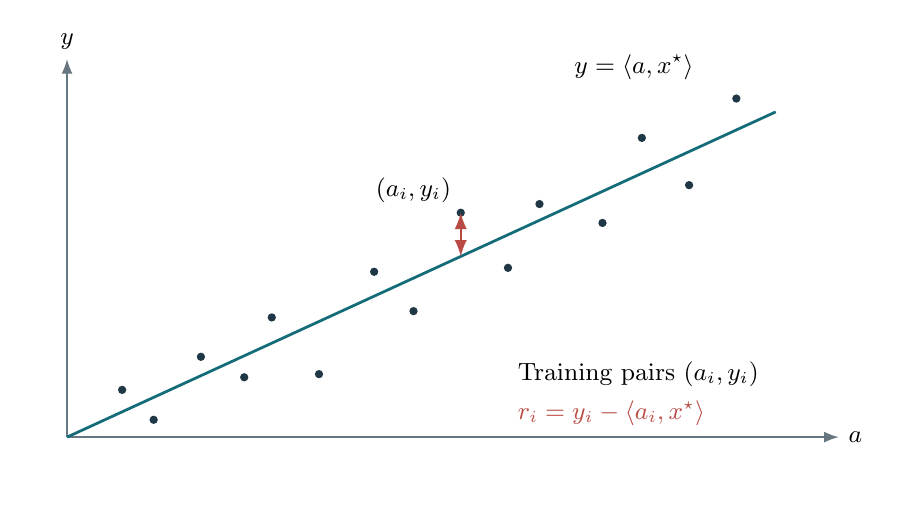
\begin{tikzpicture}
\path[use as bounding box] (-.5,-.55) rectangle (10.5,5.2);
\draw[axis] (0,0)--(9.8,0) node[right] {$a$};\draw[axis] (0,0)--(0,4.8) node[above] {$y$};
% The slope is sum_i a_i y_i / sum_i a_i^2 for the fifteen points below.
\pgfmathsetmacro{\fitslope}{0.458939197596529}
\draw[curve] (0,0)--(9,{9*\fitslope});
\node at (7.2,4.7) {$y=\langle a,x^\star\rangle$};
\node[anchor=west] at (5.6,.8) {Training pairs $(a_i,y_i)$};
\node[anchor=west,signalred] at (5.6,.3) {$r_i=y_i-\langle a_i,x^\star\rangle$};
\fill[ink] (0.7,0.6) circle (1.5pt);
\fill[ink] (1.1,0.22) circle (1.5pt);
\fill[ink] (1.7,1.02) circle (1.5pt);
\fill[ink] (2.25,0.76) circle (1.5pt);
\fill[ink] (2.6,1.52) circle (1.5pt);
\fill[ink] (3.2,0.8) circle (1.5pt);
\fill[ink] (3.9,2.1) circle (1.5pt);
\fill[ink] (4.4,1.6) circle (1.5pt);
\fill[ink] (5,2.85) circle (1.5pt);
\fill[ink] (5.6,2.15) circle (1.5pt);
\fill[ink] (6,2.96) circle (1.5pt);
\fill[ink] (6.8,2.72) circle (1.5pt);
\fill[ink] (7.3,3.8) circle (1.5pt);
\fill[ink] (7.9,3.2) circle (1.5pt);
\fill[ink] (8.5,4.3) circle (1.5pt);
\draw[signalred,<->,line width=.65pt] (5,{5*\fitslope})--(5,2.85);
\node[above left] at (5,2.85) {$(a_i,y_i)$};
\end{tikzpicture}
\end{document}
